\chapter{ILOG CPLEX}
In questa sezione verranno approfondite alcune funzioni di CPLEX necessarie ad implementare gli algoritmi descritti nei capitoli precedenti.

\section{Funzionamento}
Per poter utilizzare gli algoritmi di risoluzione forniti da CPLEX è necessario costruire il modello matematico del problema, legato all'istanza precedentemente descritta.\\
CPLEX ha due meccanismi di acquisizione dell'istanza:
\begin{enumerate}
\item{\textbf{modalità interattiva:}\\
in cui il modello viene letto da un file precedentemente generato (\textit{model.lp})}
\item{\textbf{creazione nel programma:}\\
il modello viene creato attraverso le API del linguaggio usato per la scrittura del programma}
\end{enumerate}

Le strutture utilizzate da CPLEX sono due (vedi Figura \ref{strutture_cplex}):
\begin{itemize}
\item{\textbf{ENV (enviroment):} contiene i parametri necessari all'esecuzione e al salvataggio dei risultati}
\item{\textbf{LP:} contiene il modello che viene analizzato da CPLEX durante la computazione del problema di ottimizzazione}
\end{itemize}

\begin{figure}[h] 
\begin{center} 
  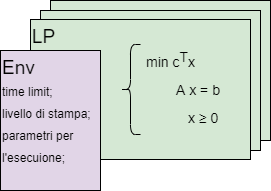
\includegraphics[scale=0.7]{Images/cplex_structs}\\ 
  \caption{\footnotesize{Strutture CPLEX}}
  \label{strutture_cplex} 
\end{center} 
\end{figure}

Ad ogni ENV è possibile associare più LP, in modo da poter risolvere in parallelo più problemi di ottimizzazione, ma nel nostro caso ne sarà sufficiente solo uno.\\
Per convenzione è stato deciso di etichettare i rami $(i,j)$ dell'istanza rispettando la proprietà $i<j$. In Figura \ref{Indici_matrice} è riportato lo schema degli indici che vengono utilizzati per etichettare le variabili.\\
In questa figura le celle $(i,j)$ bianche, sono quelle effettivamente utilizzate per indicare un arco secondo la convenzione. Il numero all'interno di queste caselle rappresenta invece l'ordine in cui queste variabili vengono inserite nel modello e quindi gli indici associati da CPLEX per accedere alla soluzione.\\Il modello così strutturato richiede però l'inserimento di un esponenziale numero di vincoli per l'eliminazione dei sub-tour, vengono quindi ora descritti altri modelli che ovvino a questo problema.
\begin{figure}[h] 
\begin{center} 
  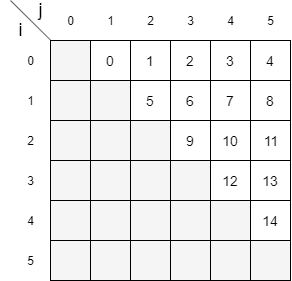
\includegraphics[scale=0.6]{Images/indices_matrix}\\ 
  \caption{\footnotesize{Indici della matrice}}
  \label{Indici_matrice} 
\end{center} 
\end{figure}

\section{Funzioni}
\subsection{Costruzione e modifica del modello}
Per poter costruire il modello da analizzare, come prima cosa, è necessario creare un puntatore alle due strutture dati utilizzate da CPLEX.
\lstinputlisting[caption={\footnotesize{modelTSP.txt}}, style=code, firstnumber=1, firstline=27, lastline=29, label=tsp_model, language=c]{Source/modelTSP.txt}
La funzione alla riga 2 alloca la memoria necessaria e riempie la struttura con valori di default. Nel caso in cui non termini con successo memorizza un codice d'errore in \textit{\&error}.\\
La funziona invocata nella riga successiva, invece, associa la struttura LP all'ENV che gli viene fornito. Il terzo parametro passato, nell'esempio "TSP", sarà il nome del modello creato.
Al termine di queste operazioni verrà quindi creato un modello vuoto. All'interno del nostro programma per inizializzarlo è stata costruita la seguente funzione:
\begin{center}
\begin{tabular}{c}
\begin{lstlisting}[linewidth=320pt, basicstyle=\footnotesize\sffamily,] 
void cplex_build_model(istanza_problema, env , lv);
\end{lstlisting}
\end{tabular}
\end{center}
\vspace{1cm}
\begin{table}[h]
\centering
\begin{tabular}{rl}
\textbf{istanza\_problema: } & {puntatore alla struttura che contiene} \\
&  {l'istanza del problema (letta dal file TSPlib)} \\
\textbf{env: } & {puntatore di tipo CPXENVptr alla}\\
& {struttura ENV precedentemente creata}\\
\textbf{lp: } & {puntatore di tipo CPXLPptr alla}\\
& {struttura LP  precedentemente creata}\\
\end{tabular}
\end{table}
All'interno di \textbf{cplex\_build\_model()} viene aggiunta una colonna alla volta al modello, definendo quindi anche la funzione obiettivo. Le variabili aggiunte corrispondono agli archi del grafo e per ciascuno di questi viene calcolato il costo come distanza euclidea. La funzione necessaria ad inserire colonne e definire la funzione di costo è la seguente:
\vspace{0.5cm}
\begin{center}
\begin{tabular}{c}
\begin{lstlisting}[linewidth=350pt, basicstyle=\footnotesize\sffamily,]     
CPXnewcols(env, lp, num_colonne, costi, lower_bound, 
           upper_bound, tipi_variabili, nomi_variabili);
\end{lstlisting}
\end{tabular}
\end{center}
\begin{table}[h]
\begin{tabular}{rl}
\textbf{env:} & {puntatore di tipo CPXENVptr alla}\\
& {struttura ENV precedentemente creata} \\
\textbf{lp:} & {di tipo CPXLPptr, è un puntatore alla struttura LP}\\
& {precedentemente creata}\\
\textbf{num\_colonne:} & {numero di colonne da inserire} \\    
\textbf{costi:} & {vettore dei costi relativi agli archi da inserire} \\
\textbf{lower\_bound:} & {vettore contenente i lower bound dei valori}\\
& {assumibili dalle variabili da inserire}\\              
\textbf{upper\_bound:} & {vettore contenente gli upper bound dei valori}\\
&  {assumibili dalle variabili da inserire} \\
\textbf{tipi\_variabili:} & {vettore contenente la tipologia delle variabili}\\
& da inserire\\
\textbf{nomi\_variabili:} & {vettore di stringhe contenenti i nomi}\\
& {delle variabili da inserire}
\end{tabular}
\end{table}
La generica colonna \textbf{i}, aggiunta dalla funzione, sarà definita dalle informazioni contenute all'interno della posizione \textbf{i} degli array, ricevuti come parametri. Nel programma elaborato durante il corso, viene aggiunta una colonna alla volta all'interno del modello. Per far ciò, è necessario comunque utilizzare riferimenti alle informazioni da inserire, in modo da ovviare il problema riguardante la tipologia di argomenti richiesti, che sono array. Ad esempio, nel nostro caso, la tipologia di una nuova variabile inserita sarà un riferimento al carattere \textbf{'B'}, che la identifica come binaria.\\
Per poter inserire il primo insieme di vincoli del problema\\
$$
\underset{e\in \delta(v)}\sum{\;x_e} = 2\;\;\;\;\;\;\;\;\;\;\;\;\;\;\;\;\;\;\forall\;v\in V \\\\
$$
\\
viene invece sfruttata la seguente funzione:
\begin{center}
\begin{tabular}{c}
\begin{lstlisting}[linewidth=330pt, basicstyle=\footnotesize\sffamily,]     
 CPXnewrows(env, lp, numero_righe,termini_noti,
            tipi_vincoli, range_valori, nomi_vincoli);
\end{lstlisting}
\end{tabular}
\end{center}
\begin{table}[h]
\centering
\begin{tabular}{rl}
\textbf{env:} & {puntatore di tipo CPXENVptr alla struttura ENV}\\
& {precedentemente creata}\\
\textbf{lp:} & {puntatore di tipo CPXLPptr alla struttura LP}\\
& {precedentemente creata}\\
\textbf{numero\_righe:} & {numero di righe (vincoli) da inserire}\\
\textbf{termini\_noti:} & {vettore dei termini noti dei vincoli}\\
\textbf{tipi\_vincoli:} & {vettore di caratteri che specifica il tipo di vincoli}\\
&{da inserire. Ogni carattere può assumere:}\\
&{\textit{'L'} per vincolo $\leq$}\\
&{\textit{'E'} per vincolo $=$}\\
&{\textit{'G'} per vincolo $\geq$}\\
&{\textit{'R'} per vincolo definito in un intervallo}\\
\textbf{range\_valori:} & {vettore di range per i valori di ogni vincolo}\\
& {(nel nostro caso è NULL)} \\
\textbf{nomi\_vincoli} & vettore di stringhe contenenti i nomi  \\
\end{tabular}
\end{table}
\begin{table}[h]
\centering
\begin{tabular}{rl}
& delle variabili da inserire
\end{tabular}
\end{table}
In modo analogo all'inserimento delle colonne, nel nostro programma viene aggiunta una riga alla volta nel modello. L'\textbf{i}-esima riga aggiunta corrisponderà al vincolo imposto sul nodo \textbf{i}-esimo, imponendo a 1 il coefficiente della variabile $x_{k,j}$ se $k=i$ $j=i$ per ogni variabile del modello. In questo modo però viene aggiunto un vincolo in cui è necessario cambiare i coefficienti delle variabili che ne prendono parte. Per fare ciò è necessaria la funzione:
\begin{center}
\begin{tabular}{c}
\begin{lstlisting}[linewidth=230pt, basicstyle=\footnotesize\sffamily,]     
CPXchgcoef(env, lp, i, j, new_value);
\end{lstlisting}
\end{tabular}
\end{center}
\begin{table}[h]
\centering
\begin{tabular}{rl}
\textbf{env:} & {puntatore di tipo CPXENVptr alla struttura ENV}\\
& {precedentemente creata}\\
\textbf{lp:} & {puntatore di tipo CPXLPptr alla struttura LP}\\
& {precedentemente creata}\\
\textbf{i:} & {intero che specifica l'indice della riga in cui modificare il }\\
&{coefficiente}\\
\textbf{j:} & {intero che specifica la colonna in cui si trova la variabile}\\
&{di cui modificare il coefficiente}\\
\textbf{new\_value:} & {nuovo valore del coefficiente}\\
\end{tabular}
\end{table}
L'utilizzo di questa metodo per inserire nuovi vincoli è però considerato inefficiente. Al suo posto è consigliato l'utilizzo di una funzione che inserisca il vincolo con già i coefficienti delle variabili impostati al valore corretto:\\
\begin{center}
\begin{tabular}{c}
\begin{lstlisting}[linewidth=385pt, basicstyle=\footnotesize\sffamily,]     
CPXaddrows(env, lp, num_nc, num_nr, nnz, const_term, type_costr,
           rmatbeg, rmatind, rmatval, col_name, row_name);
\end{lstlisting}
\end{tabular}
\end{center}
\begin{table}[h]
\centering
\begin{tabular}{rl}
\textbf{env:} & {puntatore di tipo CPXENVptr alla struttura ENV}\\
& {precedentemente creata}\\
\end{tabular}
\end{table}
\begin{table}[h]
\centering
\begin{tabular}{rl}
\textbf{lp:} & {puntatore di tipo CPXLPptr alla struttura LP}\\
& {precedentemente creata}\\
\textbf{num\_nc:} & {numero di nuove colonne che devono essere aggiunte}\\
\textbf{num\_nr:} & {numero di nuove righe che devono essere aggiunte}\\
\textbf{nnz:} & {numero di coefficienti non nulli nel vincolo aggiunto}\\
\textbf{const\_term:} & {vettore con i termini noti per ogni vincolo da aggiungere}\\
\textbf{type\_costr:} & {vettore con il tipo di vincoli da aggiungere,}\\
&{scelto tra:}\\
&{\textit{'L'} per vincolo $\leq$}\\
&{\textit{'E'} per vincolo $=$}\\
&{\textit{'G'} per vincolo $\geq$}\\
&{\textit{'R'} per vincolo definito in un intervallo}\\
\textbf{rmatbeg:} & {vettore per definire le righe da aggiungere}\\
\textbf{rmatind:} & {vettore per definire le righe da aggiungere}\\
\textbf{rmatval:} & {vettore per definire le righe da aggiungere}\\
\textbf{col\_name:} & {vettore contenente i nomi delle nuove colonne}\\
\textbf{row\_name:} & {vettore contenente i nomi dei nuovi vincoli}\\
\end{tabular}
\end{table}
\vspace{4cm}
Per rimuovere invece delle righe, viene utilizzata la seguente funzione:
\begin{center}
\begin{tabular}{c}
\begin{lstlisting}[linewidth=385pt, basicstyle=\footnotesize\sffamily,]     
CPXdelrows( CPXCENVptr env, CPXLPptr lp, int begin, int end );
\end{lstlisting}
\end{tabular}
\end{center}
\begin{table}[h]
\centering
\begin{tabular}{rl}
\textbf{env:} & {puntatore di tipo CPXENVptr alla struttura ENV}\\
& {precedentemente creata}\\
\textbf{lp:} & {puntatore di tipo CPXLPptr alla struttura LP}\\
& {precedentemente creata}\\
\end{tabular}
\end{table}
\begin{table}[h]
\centering
\begin{tabular}{rl}
\textbf{begin:} & {indice numerico della prima riga}\\
& {da cancellare}\\
\textbf{end:} & {indice numerico dell'ultima riga}\\
& {da cancellare}\\
\end{tabular}
\end{table}
\vspace{6cm} 
\subsection{Calcolo della soluzione}
Per ottenere la soluzione ottima del problema di ottimizzazione del problema correlato al modello definito in cplex, vengono utilizzate due fasi:
\begin{itemize}
\item{\textbf{Risoluzione del problema di ottimizzazione}\\
\begin{center}
\begin{tabular}{c}
\begin{lstlisting}[linewidth=120pt, basicstyle=\footnotesize\sffamily,]
CPXmipopt(env, lp);
\end{lstlisting}
\end{tabular}
\end{center}
\begin{table}[h]
\centering
\begin{tabular}{rl}
\textbf{env:} & {puntatore di tipo CPXENVptr alla struttura ENV}\\
& {precedentemente creata}\\
\textbf{lp:} & {puntatore di tipo CPXLPptr alla struttura LP}\\
& {precedentemente creata}\\
\end{tabular}
\end{table}
}
\item{\textbf{Ottenimento della soluzione}\\
\begin{center}
\begin{tabular}{c}
\begin{lstlisting}[linewidth=230pt, basicstyle=\footnotesize\sffamily,]
CPXgetmipx(env, lp, x, inizio, fine);
\end{lstlisting}
\end{tabular}
\end{center}
\begin{table}[h]
\centering
\begin{tabular}{rl}
\textbf{env:} & {puntatore di tipo CPXENVptr alla struttura ENV}\\
& {precedentemente creata}\\
\textbf{lp:} & {puntatore di tipo CPXLPptr alla struttura LP}\\
& {precedentemente creata}\\
\end{tabular}
\end{table}
\begin{table}[h]
\centering
\begin{tabular}{rl}
\textbf{x:} & {puntatore a un vettore di double in cui verranno salvati}\\
& {i valori delle variabili ottenuti dalla soluzione ottima}\\
\textbf{inizio:} & {primo indice della variabile di cui si vuole memorizzare}\\
& {ed analizzare il valore}\\
\textbf{fine:} & {indice dell'ultima variabile di cui si vuole memorizzare}\\
& {ed analizzare il valore}\\
\end{tabular}
\end{table}
\vspace{6cm}
Questa funzione salva in x tutte le variabili che hanno indice $i\in [inizio, fine]$ e quindi x deve essere un vettore di almeno $fine-inizio+1$ valori. Nel nostro programma, vengono analizzati i valori di tutte le variabili in gioco.\\
Per questo motivo \textbf{inizio=0} e \textbf{fine=num\_colonne - 1}\footnote{numero di variabili=CPXgetnumcols(env,lp);}\footnote{numero di vincoli=CPXgetnumrows(env,lp);}. In seguito il nostro programma analizza la correttezza della soluzione svolgendo la verifica su:
\begin{itemize}
\item{\textit{valori assunti dalle variabili}\\
ciascun $x_{i,j}$ assume valore $0$ o $1$ con una tolleranza di $\epsilon=10^{-5}$}
\item{\textit{grado di ciascun nodo}\\
il tour è composto al massimo da due archi che toccano lo stesso nodo}
\end{itemize}
}
\item{\textbf{Gap relativo}\\
La seguente funzione permette di ottenere il gap relativo della funzione obiettivo per un'ottimizzazione MIP.\\
\begin{center}
\begin{tabular}{c}
\begin{lstlisting}[linewidth=230pt, basicstyle=\footnotesize\sffamily,]
CPXgetmiprelgap( CPXCENVptr env, CPXCLPptr lp, double * gap_p);
\end{lstlisting}
\end{tabular}
\end{center}
\begin{table}[h]
\centering
\begin{tabular}{rl}
\textbf{env:} & {puntatore di tipo CPXENVptr alla struttura ENV}\\
& {precedentemente creata}\\
\textbf{lp:} & {puntatore di tipo CPXLPptr alla struttura LP}\\
& {precedentemente creata}\\
\end{tabular}
\end{table}
\begin{table}[h]
\centering
\begin{tabular}{rl}
\textbf{gap\_p:} & {puntatore a un double in cui verrà salvato il gap}
\end{tabular}
\end{table}
Per un problema di minimizzazione il gap relativo viene calcolato come:
$$\frac{bestinteger - bestobjective}{10^{-10}+|bestinteger|}$$
dove \textbf{bestinteger} è il valore restituito dalla funzione \textbf{CPXgetobjval()} mentre \textbf{bestobjective} da \textbf{CPXgetbestobjval()}.
}
\end{itemize}


\subsection{Lazy constraints}
Nel caso in cui si voglia sfruttare la possibilità di verificare se è stato rispettato un vincolo, solo al termine della computazione della soluzione, è necessario inserire un "lazy constraint". Per fare ciò viene utilizzata la seguente funzione:
\begin{center}
\begin{tabular}{c}
\begin{lstlisting}[linewidth=380pt, basicstyle=\footnotesize\sffamily,]     
CPXaddlazyconstraints(env, lp, num_vincoli, nnz, 
					termine_costante, tipo_vincolo, posizione_iniziale,
					indici, valori, nome_vincolo);
\end{lstlisting}
\end{tabular}
\end{center}
\begin{table}[h]
\centering
\begin{tabular}{rl}
\textbf{env:} & {puntatore di tipo CPXENVptr alla struttura ENV}\\
& {precedentemente creata}\\
\textbf{lp:} & {puntatore di tipo CPXLPptr alla struttura LP}\\
& {precedentemente creata}\\
\textbf{num\_vincoli:} & {numero di vincoli da inserire}\\
\textbf{nnz:} & {vettore con il numeri di variabili per ogni vincolo}\\ 
\textbf{termine\_costante:} & {vettore dei termini noti dei vincoli}\\
\textbf{tipi\_vincoli:} & {vettore di caratteri che specifica il tipo di vincoli}\\
&{da inserire. Ogni carattere può assumere:}\\
&{\textit{'L'} per vincolo $\leq$}\\
&{\textit{'E'} per vincolo $=$}\\
&{\textit{'G'} per vincolo $\geq$}\\
&{\textit{'R'} per vincolo definito in un intervallo}\\
\textbf{posizione\_iniziale:} & {vettore con le posizione iniziali dei coefficienti nei}\\
&{vincoli}\\
\textbf{indici:} & {vettore di vettori contenenti gli indici delle}\\
& {variabili appartenenti al vincolo}\\
\textbf{valori:} & {vettore di vettori con i coefficienti delle variabili }\\
&{del vincolo}\\
\textbf{nome\_vincolo:} & {vettore con i nomi dei vincoli}\\
\end{tabular}
\end{table}
In modo analogo alle due funzioni precedentemente descritte per l'aggiunta di righe e colonne, nel nostro modello viene inserito un vincolo per volta. Per impostare correttamente i coefficienti delle variabili presenti nel vincolo, vengono sfruttati i due array \textit{indici} e \textit{valori}. Come rappresentato in Figura \ref{lazy_constraints}, all'interno della posizione \textit{i}-esima del vettore di indici è presente la posizione dell'\textit{i}-esima variabile del vincolo da inserire (nell'esempio in figura $indici[i]=j$). Mentre l'\textit{i}-esima posizione del vettore di valori contiene il corrispondente  coefficiente (in questo caso $c_j$).
\begin{figure}[h] 
\begin{center} 
  % Requires \usepackage{graphicx} 
  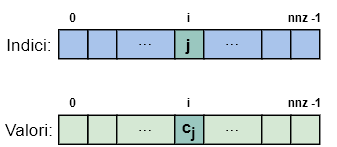
\includegraphics[scale=0.5]{Images/lazy_constraints} 
  \caption{\footnotesize{Array lazy constraints}}
  \label{lazy_constraints} 
\end{center} 
\end{figure}
\subsection{Lazy Constraint Callback}
Per poter utilizzare una lazy constraint callback, precedentemente implementata, all'interno del programma, prima di tutto è necessario installarla. Questo viene fatto attraverso la seguente funzione:
\begin{center}
\begin{tabular}{c}
\begin{lstlisting}[linewidth=380pt, basicstyle=\footnotesize\sffamily,]     
CPXsetlazyconstraintcallbackfunc(env, mylazycallback, tsp_in);
\end{lstlisting}
\end{tabular}
\end{center}
\begin{table}[h]
\centering
\begin{tabular}{rl}
\textbf{env:} & {puntatore di tipo CPXENVptr alla struttura ENV}\\
\textbf{mylazycallback:} & {puntatore di tipo CPXPUBLIC * alla callback chiamata}\\
\textbf{tsp\_in:} & {puntatore di tipo void* ad una struttura dati }\\
& {contenente le informazioni da passare alla callback}\\
\end{tabular}
\end{table}
Una volta installata la callback è necessario cambiare l'impostazione del numero di thread utilizzati dal programma. Infatti CPLEX, non sapendo se la funzione implementata dall'utente è thread safe, impedisce lo svolgimento di elaborazioni in parallelo con le callback. A meno che questo non venga esplicitamente dichiarato dall'utente con l'impostazione del corrispondente parametro.
Per questo può tornare utile la seguente funzione, che restituisce il numero di core presenti nel computer:\\
\begin{center}
\begin{tabular}{c}
\begin{lstlisting}[linewidth=170pt, basicstyle=\footnotesize\sffamily,]
CPXgetnumcores(env, ncores); 
\end{lstlisting}
\end{tabular}
\end{center}
\vspace{2cm}
\begin{table}[h]
\centering
\begin{tabular}{rl}
\textbf{env:} & {puntatore di tipo CPXENVptr ad una struttura ENV}\\
\textbf{ncores:} & {puntatore alla variabile in cui viene scritto il numero di core}\\            
\end{tabular}
\end{table} 
Come descritto nella sezione dedicata, le callback sono funzioni lasciate appositamente vuote da CPLEX, affinché l'utente possa implementarle in maniera personalizzata. Hanno però una dichiarazione standard, qui riportata: 
\begin{center}
\begin{lstlisting}[linewidth=380pt, basicstyle=\footnotesize\sffamily,]     
static int CPXPUBLIC name_function(CPXCENVptr env, void* cbdata, 
								   								int wherefrom, void* cbhandle, 	
								   								int* useraction_p)
\end{lstlisting}
\end{center}
\begin{table}[h]
\centering
\begin{tabular}{rl}
\textbf{env:} & {puntatore di tipo CPXENVptr ad una struttura ENV}\\
\textbf{cbdata:} & {puntatore che contiene specifiche informazioni per la}\\
&{callback}\\
\textbf{wherefrom:} & {contiene dove è stata invocata la callback durante} \\ 
&{l'ottimizzazione}\\
\textbf{cbhandle:} & {puntatore a dati privati dell'utente} \\
\textbf{useraction\_p:} & {specifica le azioni da eseguire al termine della callback:}\\
& {CPX\_CALLBACK\_DEFAULT: usa il nodo di CPLEX}\\
&{selezionato}\\
& {CPX\_CALLBACK\_FAIL: esci dell'ottimizzazione}\\
& {CPX\_CALLBACK\_SET: usa il nodo selezionato come}\\  
& {definito nel valore di ritorno}\\            
\end{tabular}
\end{table} 
Nell'implementarla bisogna fare particolare attenzione a renderla thread safe, se si vuole utilizzarla su più processi in parallelo. Infatti, nel caso in cui il programma lavorasse contemporaneamente con più processori, non si devono verificare interferenze di accesso agli stessi dati da parte di invocazioni diverse della callback. Quest'aspetto è lasciato a completa gestione dell'utente.\\
%CONTROLLARE COSA VUOL DIRE CPXPUBLIC
Per avere accesso alle variabili utilizzate dal nodo che invoca la callback è possibile chiamare la seguente funzione:
\begin{center}
\begin{tabular}{c}
\begin{lstlisting}[linewidth=380pt, basicstyle=\footnotesize\sffamily,]     
CPXgetcallbacknodex(env, cbdata, wherefrom, x_star, start, end);
\end{lstlisting}
\end{tabular}
\end{center}
\begin{table}[h]
\centering
\begin{tabular}{rl}
\textbf{env:} & {puntatore di tipo CPXENVptr ad una struttura ENV}\\
\textbf{cbdata:} & {puntatore che contiene specifiche informazioni per la callback}\\
\textbf{wherefrom:} & {contiene in che punto dell'ottimizzazione è stata invocata la} \\ 
&{callback}\\
\textbf{x\_star:} & {vettore in cui memorizzare le variabili} \\
\textbf{begin} & {indice della prima variabile che si vuole venga restituita}\\
\textbf{end} & {indice dell'ultima variabile che si vuole venga restituita}\\           
\end{tabular}
\end{table}
Invece, per ottenere informazioni riguardanti il problema di ottimizzazione che si sta risolvendo all'interno di una callback implementata dall'utente, è possibile utilizzare:
\begin{center}
\begin{tabular}{c}
\begin{lstlisting}[linewidth=380pt, basicstyle=\footnotesize\sffamily,]  
CPXgetcallbackinfo(env, cbdata, wherefrom, which_info, result);
\end{lstlisting}
\end{tabular}
\end{center}
\begin{table}[h]
\centering
\begin{tabular}{rl}
\textbf{env:} & {puntatore di tipo CPXENVptr ad una struttura ENV}\\
\textbf{cbdata:} & {puntatore che contiene specifiche informazioni per la callback}\\
\textbf{wherefrom:} & {contiene in che punto dell'ottimizzazione è stata invocata la}\\ 
&{callback}\\
\textbf{which\_info:} & {macro che specifica l'informazione che si desidera conoscere} \\
\textbf{result:} & {puntatore di tipo void in cui verrà memorizzata}\\          
&{l'informazione richiesta}\\
\end{tabular}
\end{table}
Macro utili da utilizzare come parametro \textit{which\_info} possono essere:
\begin{table}[h]
\centering \footnotesize
\begin{tabular}{|r|l|}
\hline
\textbf{CPX\_CALLBACK\_INFO\_MY\_THREAD\_NUM:} & {identifica il thread che }\\
&{ha eseguito la chiamata}\\
\hline
\textbf{CPX\_CALLBACK\_INFO\_BEST\_INTEGER:} & {valore della miglior}\\
&{soluzione intera}\\
\hline
\end{tabular}
\end{table}
\\Per conoscere il valore della funzione obiettivo del problema legato al nodo corrente che invoca la callback:
\begin{center}
\begin{tabular}{c}
\begin{lstlisting}[linewidth=340pt, basicstyle=\footnotesize\sffamily,]  
CPXgetcallbacknodeobjval(env, cbdata, wherefrom, objval);
\end{lstlisting}
\end{tabular}
\end{center}
\begin{table}[h]
\centering
\begin{tabular}{rl}
\textbf{env:} & {puntatore di tipo CPXENVptr ad una struttura ENV}\\
\textbf{cbdata:} & {puntatore che contiene specifiche informazioni per la callback}\\
\textbf{wherefrom:} & {contiene in che punto dell'ottimizzazione è stata invocata la} \\ 
&{callback}\\
\textbf{objval:} & {puntatore ad una variabile \textit{double} in cui memorizzare il costo} \\
\end{tabular}
\end{table}
All'interno della lazy callback è necessario aggiungere il taglio voluto al nodo corrente che la invoca. Questo può essere fatto in due diverse modalità: globale o locale.\\
Nel primo caso il vincolo aggiunto sarà visibile da tutti i nodi. Inoltre, in caso non lo ritenga più necessario, CPLEX potrà eliminarlo dal modello. Quest'operazione viene detta \textit{purge} e si verifica, ad esempio, quando un taglio non viene applicato per molte iterazioni consecutive. Per un vincolo globale viene chiamata la seguente funzione, che ne aggiunge uno alla volta:
\begin{center}
\begin{tabular}{c}
\begin{lstlisting}[linewidth=350pt, basicstyle=\footnotesize\sffamily,]  
CPXcutcallbackadd(env, cbdata, wherefrom, nnz, const_term, 
                   type_constraint, indices, values, 
                   purgeable);
\end{lstlisting}
\end{tabular}
\end{center}
\begin{table}[h]
\centering
\begin{tabular}{rl}
\textbf{env:} & {puntatore di tipo CPXENVptr ad una struttura ENV}\\
\textbf{cbdata:} & {puntatore che contiene specifiche informazioni per la}\\
&{callback}\\
\textbf{wherefrom:} & {contiene in che punto dell'ottimizzazione è stata} \\ 
&{invocata la callback}\\
\textbf{nnz:} & {numero di coefficienti non nulli} \\
\textbf{const\_term:} & {valore del termine noto} \\
\textbf{type\_constraint:} & {tipologia del taglio da aggiungere, a scelta tra} \\
&{\textit{'L'} per vincolo $\leq$}\\
&{\textit{'E'} per vincolo $=$}\\
&{\textit{'G'} per vincolo $\geq$}\\
\textbf{indices:} & {vettore contente gli indici dei coefficienti del taglio} \\
\textbf{values:} & {vettore contenente i coefficienti delle variabili nel} \\
\end{tabular}
\end{table} 
\begin{table}[h]
\centering
\begin{tabular}{rl}
&{taglio}\\
\textbf{purgeable:} & {intero che specifica in che modo CPLEX deve } \\
&{trattare il taglio, consigliato 0}\\
\end{tabular}
\end{table}
Nella seconda modalità, locale, il taglio aggiunto sarà visibile solo ai nodi discendenti di quello che invoca la callback. Viene implementata con la seguente chiamata:
\begin{center}
\begin{tabular}{c}
\begin{lstlisting}[linewidth=380pt, basicstyle=\footnotesize\sffamily,]  
CPXcutcallbackaddlocal(env, cbdata, wherefrom, nnz, const_term,
                       type_constraint, indices, values);
\end{lstlisting}
\end{tabular}
\end{center}
\begin{table}[h]
\centering
\begin{tabular}{rl}
\textbf{env:} & {puntatore di tipo CPXENVptr ad una struttura ENV}\\
\textbf{cbdata:} & {puntatore che contiene specifiche informazioni per la}\\
&{callback}\\
\textbf{wherefrom:} & {contiene in che punto dell'ottimizzazione è stata} \\ 
&{invocata la callback}\\
\textbf{nnz:} & {numero di coefficienti non nulli} \\
\textbf{const\_term:} & {valore del termine noto} \\
\textbf{type\_constraint:} & {tipologia del taglio da aggiungere, a scelta tra} \\
&{\textit{'L'} per vincolo $\leq$}\\
&{\textit{'E'} per vincolo $=$}\\
&{\textit{'G'} per vincolo $\geq$}\\
\textbf{indices:} & {vettore contente gli indici dei coefficienti del taglio} \\
\textbf{values:} & {vettore contenente i coefficienti delle variabili nel} \\
&{taglio}\\
\end{tabular}
\end{table}

\subsection{Lazy Constraint Callback General}% cambiare titolo da Lazy Constraint Callback General a general callback
Per evitare che alcune procedure interne a CPLEX vengano disattivate nel momento dell'installazione di una callback, è possibile utilizzarla con una diversa modalità rispetto a quella descritta nella sezione precedente, detta \textit{general}. Per quest'operazione viene invocata la seguente funzione, che si occupa anche di specificare il contesto in cui invocare la callback:
\begin{center}
\begin{tabular}{c}
\begin{lstlisting}[linewidth=382pt, basicstyle=\footnotesize\sffamily,]    
CPXcallbacksetfunc (env, lp, contextmask, callback, userhandle);
\end{lstlisting}
\end{tabular}
\end{center}
\begin{table}[h]
\centering
\begin{tabular}{rl}
\textbf{env:} & {puntatore di tipo CPXENVptr ad una struttura ENV}\\
\textbf{lp:} & {puntatore di tipo CPXLPptr alla struttura LP}\\
\textbf{contextmask:} & {specifica in quali contesti deve essere invocata la callback,}\\
&{è possibile metterne in or anche più di uno e gestire poi}\\
&{i singoli casi dall'interno della funzione}\\
\textbf{callback:} & {puntatore alla callback scritta dall'utente} \\
\textbf{userhandle:} & {puntatore ad una struttura che contiene i dati da passare} \\
&{alla callback}\\
\end{tabular}
\end{table}
Il parametro \textbf{contextmask} può variare a seconda dello scopo della callback creata. Alcuni possibili valori sono:
\begin{itemize}
\item{\textbf{CPX\_CALLBACKCONTEXT\_CANDIDATE}:\\la callback verrà invocata quando viene trovata da CPLEX una nuova soluzione possibile che l'utente avrà la possibilità di rifiutare;}
\item{\textbf{CPX\_CALLBACKCONTEXT\_LOCAL\_PROGRESS}: \\la callback verrà invocata nel momento in cui un thread effettua un progresso, non ancora noto globalmente, nella soluzione del problema. In questo contesto l'utente può suggerire a CPLEX una soluzione da cui proseguire la computazione (analogamente alle heuristic callback).}\\
\end{itemize}
L'utente può specificare più contesti con una sola installazione, è sufficiente separare le macro desiderate con l'operatore or bitwise ('|').\\
La user-callback implementata deve avere questa dichiarazione:
\begin{center}
\begin{tabular}{c}
\begin{lstlisting}[linewidth=382pt, basicstyle=\footnotesize\sffamily,]    
static int CPXPUBLIC name_general_callback(CPXCALLBACKCONTEXTptr
                     context, CPXLONG contextid, void* cbhandle)
\end{lstlisting}
\end{tabular}
\end{center}
in cui
\begin{table}[h]
\centering
\begin{tabular}{rl}
\textbf{contex:} & {puntatore ad una struttura di contesto della callback}\\
%opaque callback context structure, verificare traduzione
\textbf{contextid:} & {intero che specifica il contesto in cui invocare la callback}\\
\textbf{cbhandle:} & {argomento passato alla callback nell'istallazione}\\
\end{tabular}
\end{table}
L'utente può installare una sola user-callback, ma al suo interno può distinguere il contesto in cui è stata invocata grazie al parametro \textbf{contextid}.\\
Per poter accedere alla soluzione candidata e al suo costo, deve essere presente la seguente chiamata, che è specifica per il contesto \textbf{CPX\_CALLBACKCONTEXT\_CANDIDATE}:
\begin{center}
\begin{tabular}{c}
\begin{lstlisting}[linewidth=385pt, basicstyle=\footnotesize\sffamily,]    
CPXcallbackgetcandidatepoint(context, x_star, begin, end, obj_p);
\end{lstlisting}
\end{tabular}
\end{center}
\vspace{2cm}
\begin{table}[h]
\centering
\begin{tabular}{rl}
\textbf{contex:} & {contesto, come passato alla callback scritta dall'utente}\\
\textbf{x\_star:} & {vettore dove memorizzare i valori richiesti}\\
\textbf{begin:} & {indice prima colonna richiesta}\\
\textbf{end:} & {indice dell'ultima colonna richiesta}\\
\textbf{obi\_p:} & {buffer in cui memorizzare il costo della soluzione candidata,}\\
&{può essere NULL}\\
\end{tabular}
\end{table}
Per poter scartare una soluzione, nel caso in cui violi alcuni tagli specificati nella chiamata stessa, viene utilizzata la seguente funzione. Anche questa è specifica per il contesto \textbf{CPX\_CALLBACKCONTEXT\_CANDIDATE}.
\begin{center}
\begin{tabular}{c}
\begin{lstlisting}[linewidth=365pt, basicstyle=\footnotesize\sffamily,]    
CPXcallbackrejectcandidate(context, rcnt, nnz, const_term, 
                           type_constraint, rmatbeg, rmatind,
                           rmatval);
\end{lstlisting}
\end{tabular}
\end{center}
\begin{table}[h]
\centering
\begin{tabular}{rl}
\textbf{contex:} & {contesto, come passato alla callback scritta}\\
&{dall'utente}\\
\textbf{rcnt:} & {numero di vincoli che tagliano la soluzione}\\
\textbf{nnz:} & {numero di coefficienti non nulli nel vincolo}\\
\textbf{const\_term:} & {vettore di termini noti}\\
\textbf{type\_constraint:} & {vettore con la tipologia dei vincoli specificati}\\
\textbf{rmatbeg:} & {vettore di indici che specifica dove inizia ogni}\\
&{vincolo}\\
\textbf{rmatind:} & {vettore di indici delle colonne con coefficienti non}\\
&{nulli}\\
\textbf{rmatval:} & {coefficienti non nulli delle colonne specificate}\\
\end{tabular}
\end{table}
Per suggerire a CPLEX la soluzione da cui proseguire nella computazione dev'essere utilizzata la funzione:
\begin{center}
\begin{tabular}{c}
\begin{lstlisting}[linewidth=365pt, basicstyle=\footnotesize\sffamily,]    
CPXcallbackpostheursoln (context, cnt, ind, val, obj, strat);
\end{lstlisting}
\end{tabular}
\end{center}
\begin{table}[h]
\centering
\begin{tabular}{rl}
\textbf{contex:} & {contesto, come passato alla callback scritta}\\
&{dall'utente}\\
\textbf{cnt:} & {numero di elementi nei vettori ind e val}\\
\textbf{ind:} & {vettore di indici non nulli dei valori della soluzione}\\
\textbf{val:} & {vettore di valori non nulli della soluzione, possono essere NaN}\\
&{nel caso in cui la soluzione sia parziale}\\
\textbf{obj:} & {costo della nuova soluzione}\\
\textbf{strat:} & {strategia con cui CPLEX deve completare la nuova soluzione,,}\\
&{ nel caso sia parziale, scelta tra}\\
&{\textit{CPXCALLBACKSOLUTION\_NOCHECK} affinchè CPLEX}\\ 
&{non controlli l'attuabilità della soluzione (che deve essere completa) }\\
&{\textit{CPXCALLBACKSOLUTION\_CHECKFEAS} affinchè CPLEX}\\
&{ controlli solamente se la soluzione è attuabile (la soluzione proposta }\\
&{deve essere completa)}\\
&{\textit{CPXCALLBACKSOLUTION\_PROPAGATE} affinchè CPLEX }\\
&{cerchi di completare la soluzione attraverso la propagazione del bound}\\
&{\textit{CPXCALLBACKSOLUTION\_SOLVE} affinchè CPLEX}\\ 
&{fissi le variabili specificate nella soluzione e cerchi di risolvere il risultante }\\
&{problema ridotto}\\
\end{tabular}
\end{table}
CPLEX utilizzerà la soluzione proposta dall'utente solo nel caso in cui questa abbia costo inferiore all'incumbent. 

\subsection{Algoritmi Euristici}
Per poter impostare una variabile $x_{i,j}$ ad una valore fissato è necessario rendere i suoi lower e upper bound alla quantità voluta. Per cambiare questi parametri viene utilizzata la seguente funzione: 
\begin{center}
\begin{tabular}{c}
\begin{lstlisting}[linewidth=365pt, basicstyle=\footnotesize\sffamily,]    
CPXchgbds(env, lp, num_bouds, indices, which_bound, values);
\end{lstlisting}
\end{tabular}
\end{center}
\begin{table}[h]
\centering
\begin{tabular}{rl}
\textbf{env:} & {puntatore di tipo CPXENVptr alla struttura ENV}\\
\textbf{lp:} & {puntatore di tipo CPXLPptr alla struttura LP}\\
\textbf{num\_bounds:} & {numero totale di bound da cambiare}\\
\textbf{indices:} & {vettore con gli indice delle colonne corrispondenti alle}\\
&{variabili di cui cambiare il bound}\\
\textbf{which\_bound:} & {array di caratteri che specificano il bound da modificare,}\\
&{a scelta tra:}\\
&{\textit{'U'} per upper bound}\\
&{\textit{'L'} per lower bound}\\
&{\textit{'B'} per entrambi}\\
\textbf{values:} & {vettore con i nuovi valori}\\
\end{tabular}
\end{table}
\section{Parametri}\label{param}
Con le seguenti funzioni è possibile modificare i parametri di impostazione di CPLEX, altrimenti impostati ai valori di default.
Nel caso in cui si tratti di parametri di tipo INT è necessario invocare:\\
\begin{center}
\begin{tabular}{c}
\begin{lstlisting}[linewidth=330pt, basicstyle=\footnotesize\sffamily,]     
CPXsetintparam(env, numero_parametro, nuovo_valore);
\end{lstlisting}
\end{tabular}
\end{center}
mentre se di tipo DOUBLE:\\
\begin{center}
\begin{tabular}{c}
\begin{lstlisting}[linewidth=330pt, basicstyle=\footnotesize\sffamily,]     
CPXsetdblparam(env, numero_parametro, nuovo_valore);
\end{lstlisting}
\end{tabular}
\end{center}
In entrambe le funzioni:
\begin{table}[h]
\centering
\begin{tabular}{rl}
\textbf{env:} & {puntatore di tipo CPXENVptr alla struttura ENV}\\
& {di cui si vogliono cambiare i parametri}\\
\textbf{numero\_parametro:} & {intero corrispondente al parametro da modificare}\\
& {(vedi Tabella \ref{param_table})}\\
\textbf{nuovo\_valore:} & {nuovo valore (rispettivamente intero o double)}\\
& {del parametro}\\
\end{tabular}
\end{table}

\begin{table}[h]
\centering\footnotesize
\begin{tabular}{|l|l|}
\hline
\multirow{3}{*}{\textbf{CPX\_PARAM\_EPGAP}} & {tolleranza dell'intervalo tra la migliore funzione }\\
& {obiettivo intera e la funzione obiettivo del}\\
& {miglior nodo rimanente.}\\
\hline
\multirow{3}{*}{\textbf{CPX\_PARAM\_NODELIM}} & {massimo numero di nodi da risolvere prima}\\
& {che l'algoritmo termini senza aver aggiunto l'ottimalità}\\
& {(0 impone di fermarsi alla radice).}\\
\hline
\multirow{3}{*}{\textbf{CPX\_PARAM\_POPULATELIM}} & {limita il numero di soluzioni MIP generate }\\
& {per il pool di soluzioni durante ogni chiamata alla}\\
&{procedura populate.}\\
\hline
\textbf{CPX\_PARAM\_SCRIND} & {visione o meno dei messaggi di log di CPLEX}\\
\hline
\textbf{CPX\_PARAM\_MIPCBREDLP} & {permette, dalla callback chiamata, di accedere  }\\
&{al modello originale del problema e non a quello ridotto .}\\
\hline
\textbf{CPX\_PARAM\_THREADS} & {imposta il numero massimo di thread utilizzabili. }\\
\hline
\textbf{CPX\_PARAM\_RINSHEUR} & {imposta la frequenza (ogni quanti nodi) con cui deve}\\
&{essere invocato da CPLEX l'algoritmo euristico Rins.}\\
\hline
\textbf{CPX\_PARAM\_POLISHTIME} & {imposta quanto tempo in secondi deve dedicare CPLEX}\\
&{a fare il polish della soluzione.}\\
\hline
\end{tabular}
\caption{Parametri.}\label{param_table}
\end{table}
\section{Costanti utili}
Di seguito sono riportate alcune macro utili di CPLEX, insieme ai loro corrispondenti valori:
\begin{table}[h]
\footnotesize\centering
\begin{tabular}{|r|l|}
\hline
\textbf{CPX\_ON} & {\textbf{1}}\\
{} & {valore da assegnare ad alcuni parametri per abilitarli}\\
\hline
\textbf{CPX\_OFF} & {0}\\
{} & {valore da assegnare ad alcuni parametri per disabilitarli}\\
\hline
\textbf{CPX\_INFBOUND} & {$+\infty$}\\
{} & {massimo valore intero utilizzabile in CPLEX}\\
\hline
\end{tabular}
\end{table}
